\documentclass[convert={density=1024}]{standalone}
\usepackage{amsmath, amsthm, amsfonts,mathrsfs}
\usepackage{tikz-cd, kotex}
\usepackage{../.preamble/quiver}
\usepackage{../.preamble/Operators}
\begin{document}





\end{document}


% multiplicity (Algebraic_varieties-1.png)
\begin{tikzpicture}
	\draw (-2,0)--(2,0);
	\draw[domain=-2:0, variable=\x] plot({\x}, {-\x^2});
	\draw[domain=0:2, variable=\x] plot({\x}, {\x^2});
	\fill (0,0) circle[radius=2pt];
	\draw (-9,2)--(-5,2);
	\draw (-7,0) -- (-7,4);
	\fill (-7,2) circle[radius=2pt];
	\draw (-7,-.5) node{$V(x,y)$};
	\draw (0,-.5) node{$V(y, y-x^2)$};
\end{tikzpicture}

% presheaf_morphism (Presheaves-1.png)
\begin{tikzcd}
	{\mathcal{F}(V)} & {\mathcal{G}(V)} \\
	{\mathcal{F}(U)} & {\mathcal{G}(U)}
	\arrow["{\phi(V)}", from=1-1, to=1-2]
	\arrow["{\phi(U)}"', from=2-1, to=2-2]
	\arrow[from=1-2, to=2-2]
	\arrow[from=1-1, to=2-1]
\end{tikzcd}

% presheaf_kernel-1 (Presheaves-2.png)
\begin{tikzcd}
	0 & {\ker \phi(V)} & {\mathcal{F}(V)} & {\mathcal{G}(V)} \\
	0 & {\ker\phi(U)} & {\mathcal{F}(U)} & {\mathcal{G}(U)}
	\arrow[from=1-1, to=1-2]
	\arrow[from=1-2, to=1-3]
	\arrow[from=1-3, to=1-4]
	\arrow[from=2-3, to=2-4]
	\arrow[from=2-2, to=2-3]
	\arrow[from=2-1, to=2-2]
	\arrow[from=1-3, to=2-3]
	\arrow[from=1-4, to=2-4]
	\arrow[dashed, from=1-2, to=2-2]
\end{tikzcd}

% presheaf_kernel-2 (Presheaves-3.png)
\begin{tikzcd}
	0 & {\ker\phi(W)} & {\mathcal{F}(W)} & {\mathcal{G}(W)} \\
	0 & {\ker \phi(V)} & {\mathcal{F}(V)} & {\mathcal{G}(V)} \\
	0 & {\ker\phi(U)} & {\mathcal{F}(U)} & {\mathcal{G}(U)}
	\arrow[from=2-1, to=2-2]
	\arrow[from=2-2, to=2-3]
	\arrow[from=2-3, to=2-4]
	\arrow[from=3-3, to=3-4]
	\arrow[from=3-2, to=3-3]
	\arrow[from=3-1, to=3-2]
	\arrow[from=2-3, to=3-3]
	\arrow[from=2-4, to=3-4]
	\arrow[dashed, from=2-2, to=3-2]
	\arrow[from=1-2, to=1-3]
	\arrow[from=1-3, to=1-4]
	\arrow[from=1-4, to=2-4]
	\arrow[from=1-3, to=2-3]
	\arrow[dashed, from=1-2, to=2-2]
	\arrow[from=1-1, to=1-2]
	\arrow[curve={height=45pt}, dashed, from=1-2, to=3-2, crossing over]
\end{tikzcd}

% universal_property_of_sheafification (Sheaves-1.png)
\begin{tikzcd}
	{\mathcal{F}} & {\mathcal{F}^\dagger} \\
	& {\mathcal{G}}
	\arrow[from=1-1, to=2-2]
	\arrow[from=1-1, to=1-2]
	\arrow[dashed, from=1-2, to=2-2]
\end{tikzcd}

% localization (Schemes-1.png)
\begin{tikzcd}
	A & B \\
	{A_{f(\mathfrak{p})}} & {B_\mathfrak{p}}
	\arrow["\phi", from=1-1, to=1-2]
	\arrow[from=1-1, to=2-1]
	\arrow[from=1-2, to=2-2]
	\arrow["{f^\sharp_\mathfrak{p}}"', from=2-1, to=2-2]
\end{tikzcd}

%line_with_two_origin (Schemes-2.png)
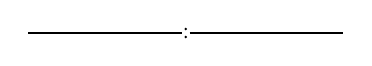
\begin{tikzpicture}
	\draw (-2,0)--(-.05,0);
	\draw (.05,0)--(2,0);
	\fill (0,0.05) circle[radius=.5pt];
	\fill (0,-.05) circle[radius=.5pt];
\end{tikzpicture}

%projective_line (Schemes-3.png)
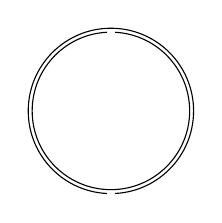
\begin{tikzpicture}
	\draw (0,0) circle[radius=1];
	\draw (0,0) circle[radius=1.05];
	\draw[white, very thick] (-.05,1)--(.05,1);
	\draw[white, very thick] (-.05,-1.05)--(.05,-1.05);
\end{tikzpicture}

% counterexamples_connectedness/irreducibility (Properties_of_schemes-1.png)
\begin{tikzpicture}
	\draw[gray!50] (-1,0)--(2,0);
	\draw (0,-1)--(0,1);
	\draw (1,-1)--(1,1);
	\draw (4,0)--(6,0);
	\draw (5,-1)--(5,1);
	\draw (5,-1.5) node{$Z(\mathrm{x}\mathrm{y})$};
	\draw (.5,-1.5) node{$Z(\mathrm{x}(\mathrm{x}-1))$};
\end{tikzpicture}

% counterexamples_reducedness (Properties_of_schemes-2.png)
\begin{tikzpicture}
	\draw[domain=-2:0, variable=\x] plot({\x}, {-\x^2});
	\draw[domain=0:2, variable=\x] plot({\x}, {\x^2});
	\draw (0,-.5) node{$Z(\mathrm{y}-\mathrm{x}^2)$};
\end{tikzpicture}

% finite_type_morphism (Properties_of_schemes-3.png)
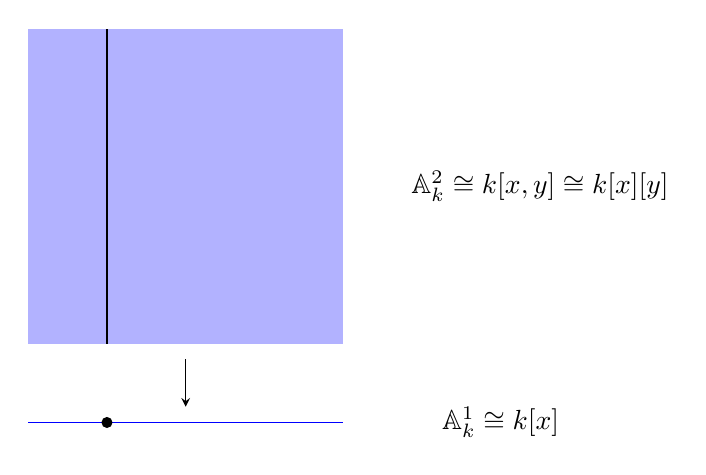
\begin{tikzpicture}
	\draw[blue] (-2,0) -- (2,0);
	\fill[blue!30] (-2,1) rectangle (2,5);
	\fill (-1,0) circle [radius=2pt];
	\draw[thick] (-1,1) -- (-1,5);
	\draw[-{stealth}] (0,0.8) -- (0,0.2);
	\draw (4.5,3) node{$\mathbb{A}^2_k\cong \Spec k[x,y]\cong \Spec k[x][y]$};
	\draw (4,0) node{$\mathbb{A}^1_k\cong \Spec k[x]$};
\end{tikzpicture}

% finite_morphism (Properties_of_schemes-4.png)
\begin{tikzpicture}
	\draw (-.1,0)--(4.9,0) node[right]{$\mathbb{A}^1_k\cong \Spec k[x]$};
	\draw[domain=0:2.2] plot (\x^2,\x)node[right]{$\Spec k[x,y]/(y^2-x)$};
	\draw[domain=0:2.2] plot (\x^2,-\x);
	\fill (4,0) circle[radius=2pt];
	\draw[dashed] (4,2)--(4,-2); 
	\fill[red] (4,2) circle[radius=2pt];
	\fill[red] (4,-2) circle[radius=2pt];
\end{tikzpicture}

% fiber_product (Properties_of_schemes-5.png)
\begin{tikzcd}
	W \\
	& {X\times_ZY} & Y \\
	& X & Z
	\arrow[dashed, from=1-1, to=2-2]
	\arrow["{q'}", curve={height=-6pt}, from=1-1, to=2-3]
	\arrow["{p'}"', curve={height=6pt}, from=1-1, to=3-2]
	\arrow["q", from=2-2, to=2-3]
	\arrow["p"', from=2-2, to=3-2]
	\arrow["g", from=2-3, to=3-3]
	\arrow["f"', from=3-2, to=3-3]
\end{tikzcd}

% diagonal_morphism (Valuative_criteria-1.png)
\begin{tikzcd}
	{X} \\
	& {X\times_YX} & X \\
	& X & Y
	\arrow[dashed, from=1-1, to=2-2]
	\arrow[curve={height=-6pt}, Rightarrow, no head, from=1-1, to=2-3]
	\arrow[curve={height=6pt}, Rightarrow, no head, from=1-1, to=3-2]
	\arrow[from=2-2, to=2-3]
	\arrow[from=2-2, to=3-2]
	\arrow["f", from=2-3, to=3-3]
	\arrow["f"', from=3-2, to=3-3]
\end{tikzcd}

% valuative_criterion_for_separatedness (Valuative_criteria-2.png)
\begin{tikzcd}
	{\Spec K} & X \\
	{\Spec R} & Y
	\arrow[from=1-1, to=1-2]
	\arrow[from=1-1, to=2-1]
	\arrow["f", from=1-2, to=2-2]
	\arrow[dashed, from=2-1, to=1-2]
	\arrow[from=2-1, to=2-2]
\end{tikzcd}

\begin{tikzcd}
	{\Spec K} & X \\
	{\Spec R} & Y
	\arrow[from=1-1, to=1-2]
	\arrow[from=1-1, to=2-1]
	\arrow["f", from=1-2, to=2-2]
	\arrow[dashed, from=2-1, to=1-2]
	\arrow[from=2-1, to=2-2]
\end{tikzcd}

\begin{tikzcd}
	X & A \\
	B & C
	\arrow["a"', from=1-2, to=1-1]
	\arrow["b", from=2-1, to=1-1]
	\arrow["f"', from=2-2, to=1-2]
	\arrow["g", from=2-2, to=2-1]
\end{tikzcd}
